\newpage

\section{Wing structural arrangement}

\subsection{Discussion of the wing structural arrangement}

The Lockheed Model 10 Electra has a complex wing structure, consisting of several elements such as the spars(2), ribs, skin and aileron. The wing structural arangement is shown in Table \ref{tab:wing_structural_arrangement}.

\begin{sidewaystable}[!htp]
    \centering
    \caption{Wing structural arrangement}
    \label{tab:wing_structural_arrangement}
    \resizebox{\textwidth}{!}{\begin{tabular}{lllllll} \toprule
    Element                             & Assembly & Load Factor            & How It Works                                                                                                           & What Does the Element Experience                     & Raw Material                                  & Load Position/Direction                                                  \\
    \midrule
    \multirow{2}{*}{Front spar}             & Cap      & Bending moment, torque & \multirow{2}{*}{Transfers lift and drag loads from the wing to the fuselage}                                           & Tension, Compression                                 & \multirow{2}{*}{High-strength aluminum alloy} & Along the longitudinal axis of the spar                                  \\
                                        & Web      & Shear force            &                                                                                                                        & Shear stress                                         &                                               & On its own surface                                                       \\
                                \midrule
    \multirow{2}{*}{Rear spar}             & Cap      & Bending moment, torque & \multirow{2}{*}{Supports the weight of the fuel tanks and transfers lift and drag loads from the wing to the fuselage} & Tension, Compression                                 & \multirow{2}{*}{High-strength aluminum alloy} & Along the longitudinal axis of the spar                                  \\
                                        & Web      & Shear force            &                                                                                                                        & Shear stress                                         &                                               & On its own surface                                                       \\
                                \midrule
%     \multirow{2}{*}{Spar 3}             & Cap      & Bending moment, torque & \multirow{2}{*}{Transfers lift and drag loads from the wing to the fuselage}                                           & Tension, Compression                                 & \multirow{2}{*}{High-strength aluminum alloy} & Along the longitudinal axis of the spar                                  \\
%                                         & Web      & Shear force            &                                                                                                                        & Shear stress                                         &                                               & On its own surface                                                       \\
%                                 \midrule
%     \multirow{2}{*}{Spar 4}             & Cap      & Bending moment, torque & \multirow{2}{*}{Transfers lift and drag loads from the wing to the wingtip and helps maintain the shape of the wing}   & Tension, Compression                                 & \multirow{2}{*}{High-strength aluminum alloy} & Along the longitudinal axis of the spar                                  \\
%                                         & Web      & Shear force            &                                                                                                                        & Shear stress                                         &                                               & On its own surface                                                       \\
%                                 \midrule
    Typical Ribs                        & Web      & Shear force            & Gives the wing its airfoil shape and provides support for the skin                                                     & Shear stress                                         & High-strength aluminum alloy                  & On its own surface                                                       \\
    \midrule
    \multirow{2}{*}{Reinforcement Ribs} & Cap      & Bending moment, torque & \multirow{2}{*}{Provides additional support to the typical ribs and helps maintain the shape of the wing}              & Tension, Compression                                 & \multirow{2}{*}{High-strength aluminum alloy} & Along the longitudinal axis of the rib                                   \\
                                        & Web      & Shear force            &                                                                                                                        & Shear stress                                         &                                               & On its own surface                                                       \\
    \midrule
    Stringers                           & -        & Bending moment, torque & Provides additional support and stiffness to the skin                                                                  & Shear stress, compression and tension                & High-strength steel                           & Perpendicular to the surface of the skin, along the axis of the stringer \\
    \midrule
    Skin                                & Skin     & Bending moment, torque & Provides an aerodynamic smooth surface to reduce drag                                                                  & Shear stress, compression and tension                & Aluminum alloy sheet                          & On its own surface                                                       \\
    \midrule
    \multirow{2}{*}{Aileron}            & Truss    & \multirow{2}{*}{-}     & \multirow{2}{*}{Provides lateral control and changes the lift distribution on the wing}                                & \multirow{2}{*}{Roll moment, bending moment, torque} & \multirow{2}{*}{High-strength aluminum alloy} & Perpendicular to the longitudinal axis of the aircraft                   \\
                                        & Skin     &                        &                                                                                                                        &                                                      &                                               & Along the chord line of the wing      \\
                                        \bottomrule                                  
    \end{tabular}}
\end{sidewaystable}

\subsection{Sketch}

Isometric view of the structure is shown in Figure \ref{fig:wing_structural_arrangement}.

\begin{figure}[!htp]
        \centering
        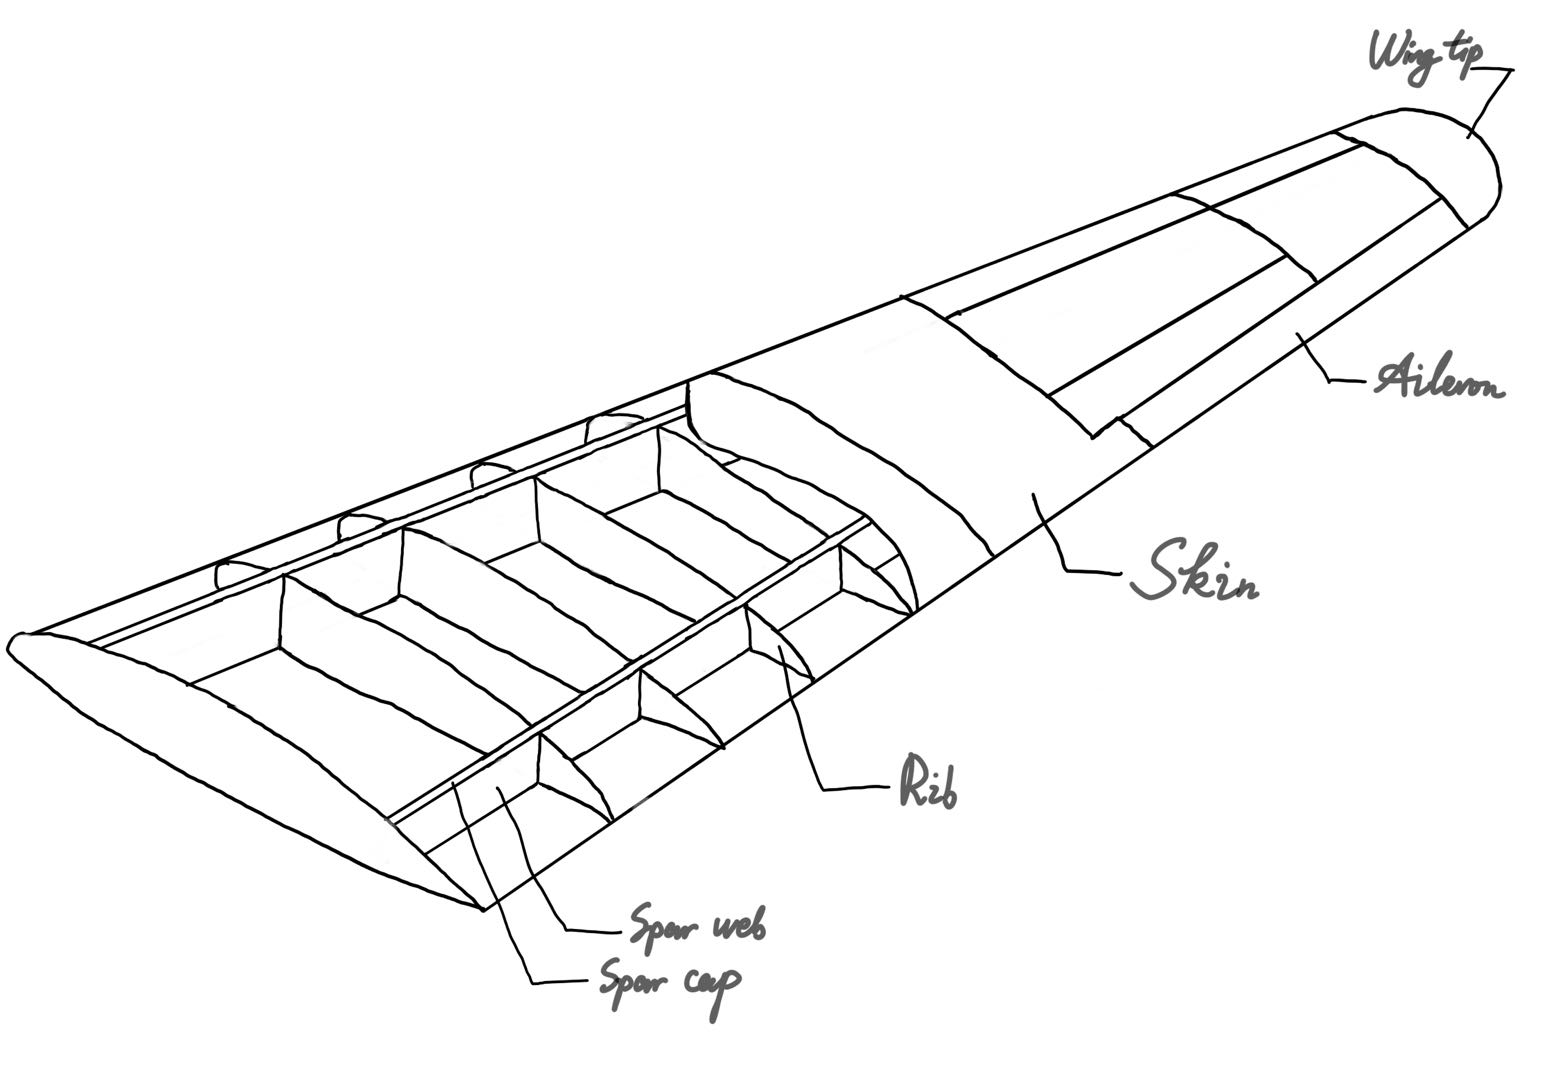
\includegraphics[width=0.9\textwidth]{images/wing structure.jpg}
        \caption{Isometric view of the wing structure of Lockheed Model 10 Electra}
        \label{fig:wing_structural_arrangement}
\end{figure}